% !TeX encoding = UTF-8
% !TeX spellcheck = pl_PL

% $Id:$

\documentclass[10pt, a
4paper]{article}
\usepackage[utf8]{inputenc}
\usepackage[polish]{babel}
\usepackage{multirow}
\usepackage{caption}
\usepackage{bigdelim}
\usepackage{bigstrut}
\usepackage[ampersand]{easylist}
\usepackage{graphicx}

\usepackage{listings}
\usepackage{xcolor} % for setting colors
% set the default code style
\lstset{
    frame=tb, % draw a frame at the top and bottom of the code block
    tabsize=4, % tab space width
    showstringspaces=false, % don't mark spaces in strings
    numbers=left, % display line numbers on the left
    commentstyle=\color{green}, % comment color
    keywordstyle=\color{blue}, % keyword color
    stringstyle=\color{red} % string color
}


\newcommand{\doctype}{Opracowanie zagadnień}
\newcommand{\projectname}{Sterowanie procesami dyskretnymi}

\newcommand{\osobaA}{J\k{e}drzej Bara\'nski}
\newcommand{\osobaB}{Dawid Zaraza}
\newcommand{\osobaC}{Grzegorz Ludwa}
\newcommand{\osobaD}{Rafał Mecwaldowski}
\newcommand{\osobaE}{Michał Wieczorek}
\newcommand{\osobaF}{}

%Preambuła dokumentu

% linki w spisie tresci, bibliografi
\usepackage[bookmarks=true,bookmarksnumbered=false,unicode=true,pdftex=true, colorlinks,filecolor=black,linkcolor=black,urlcolor=black,citecolor=black]{hyperref}

%ustawienie rozmiaru papieru
\usepackage[a4paper, left=2.5cm, right=2.5cm, top=2.5cm, bottom=2.5cm, headsep=1.2cm]{geometry}

%rozmaite ustawienia pozwalające okreslić język

%NALEŻY wybrać jeden z pakietów
%\usepackage{polski} %przydatne podczas składania dokumentów w j. polskim
\usepackage[polish]{babel}  % pakiet lokalizujący dokument w języku polskim
%\usepackage[british]{babel}

\usepackage{indentfirst}	% polski styl pisania (np. rozpoczecie pierwszego akapitu
% pod nazwa rozdzialu od wciecia)
%\usepackage[OT4]{fontenc}
\usepackage[utf8]{inputenc} % w miejsce utf8 można wpisać latin2 bądź cp1250,
% w zależności od tego w jaki sposób kodowane są 
% polskie znaki diakrytyczne przy wprowadzaniu 
% z klawiatury.
%kodowanie znaków, zależne od systemu
\usepackage[T1]{fontenc} %poprawne składanie polskich czcionek

%OPEROWANIE NA OBRAZACH
\usepackage{graphicx}       % pakiet graficzny, umożliwiający m.in.
% import grafik w formacie eps
%\usepackage{epstopdf}		% pozwala na importowanie grafik w formacie eps
% przy użyciu pdflatex
\usepackage[update,prepend]{epstopdf}
\usepackage{rotating}       % pakiet umożliwiający obracanie rysunków
\usepackage{subfigure}      % pakiet umożliwiający tworzenie podrysunków
\usepackage{epic}           % pakiet umożliwiający rysowanie w środowisku latex
\usepackage{psfrag}         % pakiet umożliwiający podmianę łańcuchów znaków 
% w plikach eps
%\usepackage{curves}         % pakiet do wykreslania krzywych

%pakiety dodające dużo dodatkowych poleceń matematycznych
\usepackage{amsfonts}       % pakiet z rozmaitymi czcionkami matematycznymi
%\usepackage{amssymb}        % pakiet z rozmaitymi symbolami matematycznymi
\usepackage{amsmath}        % pakiet z rozmaitymi środowiskami matematycznymi

\usepackage{fp}             % pakiet z funkcjami operujacymi 
% na liczbach zmiennoprzecinkowych
\usepackage{calc}           % pakiet umożliwiający operacje arytmetyczne
% na tzw. licznikach (liczbach całkowitych)
\usepackage{leftidx}		% indeksy górne i dolne po lewej stronie

%definicje matematyczne
\providecommand{\abs}[1]{\lvert#1\rvert}
\providecommand{\norm}[1]{\lVert#1\rVert}

%pakiety wspomagające i poprawiające składanie tabel
\usepackage{supertabular}
\usepackage{array}
\usepackage{tabularx}
\usepackage{hhline}
\usepackage{longtable}		% wsparcie dla dlugich tabel
\usepackage{multicol}		% podzial strony na wiele kolumn
\usepackage{booktabs}
\usepackage{tabu}

%pakiet do BibTex
\usepackage{cite}

\usepackage{url} %pakiet pozawalający na dodawanie adresów url w bibliografi

%pakiet wypisujący na marginesie etykiety równań i rysunków zdefiniowanych przez \label{}, chcąc wygenerować finalną wersję dokumentu wystarczy usunąć poniższą linię
%\usepackage{showlabels}

\usepackage{float}			% lepsza obsluga mechanizmow obiektow plywajacych
% wymuszenie wstawienia np. tabeli, obrazka w danym miejscu przez [H]

\usepackage{listings}       % pakiet dedykowany zrodlom programow
\usepackage{color}


\usepackage{graphicx}	% do gifów



\definecolor{dkgreen}{rgb}{0,0.6,0}
\definecolor{gray}{rgb}{0.5,0.5,0.5}
\definecolor{mauve}{rgb}{0.58,0,0.82}

\lstset{ %
	language=Matlab,                % the language of the code
	basicstyle=\scriptsize,           % the size of the fonts that are used for the code
	numbers=left,                   % where to put the line-numbers
	numberstyle=\tiny\color{gray},  % the style that is used for the line-numbers
	stepnumber=1,                   % the step between two line-numbers. If it's 1, each line 
	% will be numbered
	numbersep=5pt,                  % how far the line-numbers are from the code
	backgroundcolor=\color{white},      % choose the background color. You must add \usepackage{color}
	showspaces=false,               % show spaces adding particular underscores
	showstringspaces=false,         % underline spaces within strings
	showtabs=false,                 % show tabs within strings adding particular underscores
	%frame=single,                   % adds a frame around the code
	rulecolor=\color{black},        % if not set, the frame-color may be changed on line-breaks within not-black text (e.g. comments (green here))
	tabsize=2,                      % sets default tabsize to 2 spaces
	captionpos=b,                   % sets the caption-position to bottom
	breaklines=true,                % sets automatic line breaking
	breakatwhitespace=false,        % sets if automatic breaks should only happen at whitespace
	%title=\lstname,                   % show the filename of files included with \lstinputlisting;
	% also try caption instead of title
	keywordstyle=\color{blue},          % keyword style
	commentstyle=\color{dkgreen},       % comment style
	stringstyle=\color{mauve},         % string literal style
	escapeinside={\%*}{*)},            % if you want to add LaTeX within your code
	morekeywords={*,...},              % if you want to add more keywords to the set
	deletekeywords={...}              % if you want to delete keywords from the given language
}

%polish signs in lst code
\lstset{literate=%
	{ą}{{\k{a}}}1
	{ć}{{\'c}}1
	{ę}{{\k{e}}}1
	{ł}{{\l}}1
	{ń}{{\'n}}1
	{ó}{{\'o}}1
	{ś}{{\'s}}1
	{ż}{{\.z}}1
	{ź}{{\'z}}1
	{Ą}{{\k{A}}}1
	{Ć}{{\'C}}1
	{Ę}{{\k{E}}}1
	{Ł}{{\L}}1
	{Ń}{{\'N}}1
	{Ó}{{\'O}}1
	{Ś}{{\'S}}1
	{Ż}{{\.Z}}1
	{Ź}{{\'Z}}1
}

\usepackage{verbatim}       % pakiet dedykowany rozmaitym wydrukom tekstowym
\usepackage{ifthen}         % pakiet umożliwiający tworzenie prostych programów
% (m.in. zawiera instrukcje powtórzeniowe 
% i warunkowe)
\usepackage{upquote}		%normal quotations marks ' and `

% deklaracje wymagane przez pakiet theorem automatycznie ladowany w przypadku
% klasy dokumentu article
%
\newtheorem{Dn}{Definicja}[section]     % deklaracja srodowiska definicja
\newtheorem{La}[Dn]{Lemat}                % deklaracja srodowiska lemat
\newtheorem{Tm}[Dn]{Twierdzenie}          % deklaracja srodowiska twierdzenie
\newtheorem{Rk}[Dn]{Spostrze{\.z}enie}  % deklaracja srodowiska spostrzezenie
\newtheorem{Am}[Dn]{Algorytm}           % deklaracja srodowiska algorytm
\newtheorem{As}[Dn]{Za{\l}o{\.z}enie}   % deklaracja srodowiska zalozenie
\newtheorem{Pn}[Dn]{Propozycja}           % deklaracja srodowiska propozycja
\newtheorem{Py}[Dn]{W{\l}asno{\'s}{\'c}}  % deklaracja srodowiska wlasnosc
\newtheorem{Cy}[Dn]{Wniosek}              % deklaracja srodowiska wniosek
\newtheorem{Ee}[Dn]{Przyk{\l}ad}        % deklaracja srodowiska przyklad
\newtheorem{Ex}{{\'C}wiczenie}          % deklaracja srodowiska cwiczenie

%helps to specify width of a column in table
%\begin{tabular}{|C{1cm}|c|c|c|c|c|c|c|c|c|c|}
%first column will have widht of 1cm
\newcolumntype{L}[1]{>{\raggedright\let\newline\\\arraybackslash\hspace{0pt}}m{#1}}
\newcolumntype{C}[1]{>{\centering\let\newline\\\arraybackslash\hspace{0pt}}m{#1}}
\newcolumntype{R}[1]{>{\raggedleft\let\newline\\\arraybackslash\hspace{0pt}}m{#1}}

\sloppy			%zawija bardzo długie linie

%\pagenumbering{gobble}% Remove page numbers (and reset to 1)

\begin{document}

\def\tablename{Tabela}	%zmienienie nazwy tabel z Tablica na Tabela

\begin{titlepage}
	\begin{center}
		\rule{\textwidth}{0.08cm}\\[0.4cm]
		{\huge \bfseries \doctype}\\[1cm]
		{\huge \bfseries \projectname}\\[0.5cm]
		\rule{\textwidth}{0.08cm}\\[1cm]
        
        \begin{flushright} \large
		\emph{Autorzy:}\\
		\osobaA\\
        \osobaB\\
        \osobaC\\
        \osobaD\\
        \osobaE\\
        [0.4cm]
		\end{flushright}

		\vfill
		
		{\large \today}
	\end{center}	
\end{titlepage}

\newpage
\tableofcontents
\newpage


\section{Przykładowe zadania optymalizacji. Klasyfikacja podejść i metod}
\subsection{Opis} 
Optymalizacja --- metoda wyznaczania najlepszego (optymalnego) rozwiązania (poszukiwanie ekstremum funkcji) z punktu widzenia określonego kryterium (wskaźnika) jakości (np. kosztu, drogi, wydajności).\\
Rozwiązanie spełniające wszystkie ograniczenia występujące w problemie nazywamy \textbf{rozwiązaniem dopuszczalnym}.

\indent Stosuje się optymalizacje jedno i wielokryterialne. Optymalizacja wielokryterialna występuje w~wielu różnych dziedzinach: w projektowaniu produktu i procesu produkcji, finansów, projektowaniu samolotów, w przemyśle chemicznym, projektowaniu samochodów, wszędzie tam, gdzie optymalne decyzje muszą być podjęte w obecności kompromisów pomiędzy dwoma lub więcej sprzecznymi celami. Przykładem wielokryterialnej optymalizacji jest maksymalizacja zysków i minimalizacji kosztów produktu, maksymalizacja wydajności przy ograniczaniu zużycia paliwa pojazdu, czy też obniżenie masy urządzenia przy jednoczesnej maksymalizacji wytrzymałości poszczególnych jego 
komponentów.\\
\subsection{Przykłady}
\begin{itemize}
\item Planowanie produkcji
\item Projektowanie UAR( znaleźć wartości nastaw regulatora w zbiorze dopuszczalnym dla których funkcja oceny (całka z uchybu) przyjmuje  najmniejszą wartość na tym zbiorze
\item Zadanie identyfikacji modelu
\item Zadanie lokalizacji
\item kolekcjonowanie zamówień, 
\item rozkroju płyt (aby jak najmniej odpadów), 
\item zarządzania kontenerami (żeby nie transportować pustych kontenerów po globie), linia montażowa
\end{itemize}

\subsection{Klasyfikacja podejść i metod}
\begin{enumerate}
\item Dane losowe o znanym lub nieznanym rozkładzie
\begin{itemize}
\item Procesy stochastyczne
\item Teoria kolejek
\item Analiza systemów kolejkowych
\item Masowa obsługa
\item Optymalizacja stochastyczna
\end{itemize}
\item Dane deterministyczne (cykliczne)
\begin{itemize}
\item Sieci Petriego
\item Discrete Event System (EDS)
\item Optymalizacja dyskretna
\end{itemize}
\item Dane rozmyte
\begin{itemize}
\item Analiza rozmyta
\end{itemize}
\end{enumerate}

\newpage
\textbf{Metody dokładne:}
\begin{itemize}
\item Efektywne algorytmy dedykowane
\item Schemat podziału i ograniczeń (B\&B)
\item Schemat programowania dynamicznego
\item Programowanie liniowe całkowitoliczbowe
\item Programowanie liniowe binarne (PLB)
\item Metody subgradientowe
\end{itemize}
\textbf{Metody przybliżone:}
\begin{enumerate}
\item konstrukcyjne
\item reguły priorytetowe
\item adaptacja rozwiązania otrzymanego dla rozwiązania zrelaksowanego
\item przybliżenie rozwiązania rozwiązaniem otrzymanym z pokrewnych problemów
\item poprawiające
\end{enumerate}


\subsection{Optymalizacja statyczna i dynamiczna}
\begin{itemize}
\item \textbf{optymalizację statyczną} (sprowadzającą się do poszukiwania ekstremum funkcji),
\item \textbf{optymalizację dynamiczną} (sprowadzającą się do poszukiwania ekstremum funkcjonału).
\end{itemize}
\subsubsection{Optymalizacja statyczna}
Optymalizacja statyczna zajmuje się poszukiwaniem optymalnego punktu pracy, czyli takiego, w którym wartość funkcji celu jest najlepsza. Zależnie od sformułowania zadania będzie to wartość największa i najmniejsza, ale zawsze ekstremalna. Poszukiwanie ekstremum może się odbywać w pewnym ograniczonym obszarze zawierającym tylko jedno ekstremum - mówimy wówczas o poszukiwaniu ekstremum lokalnego. Może też odbywać się w całej przestrzeni argumentów i wówczas mówimy o poszukiwaniu ekstremum globalnego.\\
\indent Zadanie nie zawsze udaje się rozwiązać poprawnie. Mimo bowiem istnienia ekstremum globalnego procedura poszukiwania może się zakończyć w punkcie będącym ekstremum lokalnym. Większość algorytmów numerycznych to algorytmy poszukiwania ekstremum lokalnego. Skuteczność działania takich procedur jest więc w dużym stopniu uwarunkowana wyborem odpowiedniego punktu startowego.\indent
Wśród metod optymalizacji statycznej wyróżnia się dwie zasadnicze grupy: \textbf{programowanie liniowe i programowanie nieliniowe}. Programowanie liniowe polega na poszukiwaniu ekstremum liniowej funkcji celu przy ograniczeniach będących również funkcjami liniowymi. W zagadnieniach programowania liniowego ekstremum jest zawsze globalne w danym obszarze poszukiwań. Programowanie nieliniowe polega na poszukiwaniu ekstremum funkcji celu dowolnej postaci, przy ograniczeniach będących również wyrażonymi przez dowolne funkcje.
\subsubsection{Optymalizacja dynamiczna}
Typowe zagadnienie optymalizacji dynamicznej polega na poszukiwaniu takiego ciągu decyzji w danym przedziale czasu, który zapewni ekstremum pewnego wskaźnika jakości zależącego od przebiegu zmian tej decyzji, określanym na całym przedziale czasu. Wskaźnik jakości jest więc funkcjonałem tej decyzji, określanym na danym przedziale czasu.


\subsection{Klasyfikacja zadań optymalizacji ze względu na trudność znajdowania ich rozwiązania}
\begin{itemize}
\item I Podział
\begin{itemize}
\item Zadania bez ograniczeń - wszystkie warianty są dopuszczalne,
\item Zadania z ograniczeniami - zadania, w których określono zbiór wariantów dopuszczalnych.
\end{itemize}
\item II Podział
\begin{itemize}
\item Zadania liniowe - wszystkie funkcje określające są afiniczne(Zadania liniowe mają zawsze ograniczenia),
\item Zadania nieliniowe - co najmniej jedna funkcja nie jest afiniczna
\end{itemize}
\item III Podział
\begin{itemize}
\item Zadania gładkie klasy $C^n$ - gdzie n jest rzędem ciągłej pochodnej funkcji f,$g_{i}$,$h_{k}$ mającej ją najniższą,
\item Zadania nieróżniczkowalne - gdy co najmniej jedna funkcja zadania nie jest różniczkowalna,
\end{itemize}
\item IV Podział
\begin{itemize}
\item Zadania wypukłe - gdy funkcja wyboru f i zbiór dopuszczalny D są wypukłe,
\item Zadania niewypukłe - analogicznie
\end{itemize}
\end{itemize}





\newpage
\section{Optymalizacja procesu wytwarzania. Szeregowanie}
\subsection{Harmonogramy}
\noindent \textbf{Harmonogramowanie produkcji polega na:}
\begin{itemize}
\item rozłożeniu w czasie przydziału zasobów (materiały, maszyny, kapitał) do zleceń produkcyjnych,
\item podziale zadań (zleceń (montaż, obróbka)) na partie produkcyjne,
\item określeniu terminów rozpoczęcia i zakończenia realizacji partii produkcyjnych na poszczególnych maszynach.
\end{itemize}

\noindent \textbf{Kryteria optymalności harmonogramu produkcji reprezentują kompromis pomiędzy:}
\begin{itemize}
\item kosztami niedotrzymania terminów,
\item zaspokojenia zapotrzebowania,
\item kosztami utrzymywania zapasów i kosztami częstych zmian asortymentu produkcji.
\end{itemize}
\noindent \textbf{Kryteria oceny harmonogramu, np.:}
\begin{itemize}
\item długość uszeregowania,
\item średni czas przepływu,
\item maksymalne opóźnienie,
\item średnie spóźnienie.
\end{itemize}

\subsection{Szeregowanie zadań}
\noindent \textbf{Klasyczną metodą harmonogramowania produkcji jest szeregowanie zadań.}

W systemie składającym się z M stanowisk roboczych (maszyn) należy wykonać N zleceń (zadań). Każde zlecenie jest poleceniem wykonania określonej liczby sztuk produktu o numerze $j=j_{n}$.
Proces wytwarzania produktu j składa się z operacji o numerach k należące do $K_{j}$. Zadanie jest poleceniem jednokrotnego bądź wielokrotnego wykonania danej operacji. Operacje należące do procesu wytwarzania dowolnego produktu muszą być wykonywane w określonej kolejności. Zadania są wykonywane na~stanowiskach roboczych:
\begin{itemize}
\item równoległych (spełniających te same funkcje),
\item dedykowanych (różniących się wykonywanymi funkcjami).
\end{itemize}

\noindent \textbf{Szeregowanie zadań:}
\begin{enumerate}
\item \textbf{F --- przepływowy (flow shop)}, Rys. 1, w którym wszystkie zadania posiadają jednakową marszrutę technologiczną, wymagają obsługi na
wszystkich stanowiskach, zaś każde stanowisko wymaga określenia odpowiedniej
sekwencji wprowadzania zadań,
\item \textbf{F* --- przepływowy permutacyjny (permutation flow-shop)}, Rys. 1, które ma takie same założenia jak F z dodatkowym wymaganiem aby kolejność
obsługi zadań na wszystkich maszynach była jednakowa (zgodna
z kolejnością wprowadzania zadań do systemu),
\item \textbf{J --– gniazdowy (job-shop)}, Rys. 2, w którym różne zadania mogą posiadać różne (co do liczby jak i kolejności odwiedzania stanowisk) marszruty
technologiczne,
\item \textbf{G –-- ogólny (general-shop)}, w którym każde zadanie jest pojedynczą operacją ($o_i$ = 1), zaś zależności technologiczne są dane dowolnym grafem,
\item \textbf{I --- równoległy (parallel shop)}, Rys. 3, w którym każde zadanie jest pojedynczą operacją oraz wszystkie operacje są wykonywane na dokładnie jednej z kilku równoległych (tego samego typu) maszyn,
\item \textbf{O --- otwarty (open shop)}, w którym wszystkie operacje zadania mają być wykonane lecz kolejność technologiczna operacji w zadaniu nie jest
określona.
\end{enumerate}

\begin{figure}[H]
\begin{center}
\label{diagram}
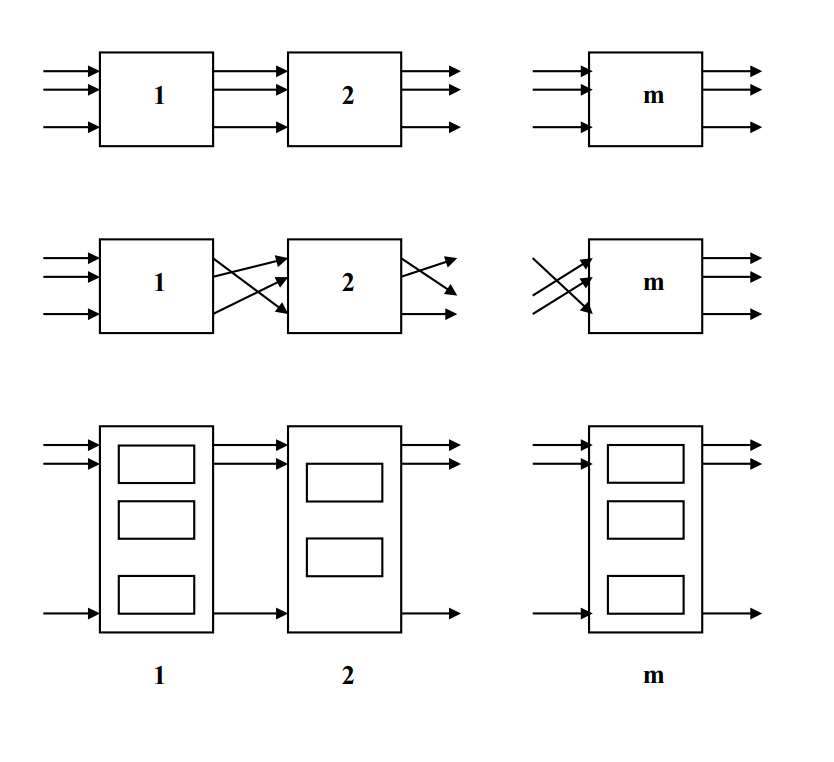
\includegraphics[scale = 0.5]{Rysunki/szeregowanie.png}
\caption{Struktury przepływowych systemów produkcyjnych: permutacyjny
(F*), niepermutacyjny (F), z maszynami równoległymi w stanowisku (PF).}
\end{center}
\end{figure}

\begin{figure}[H]
\begin{center}
\label{diagram}
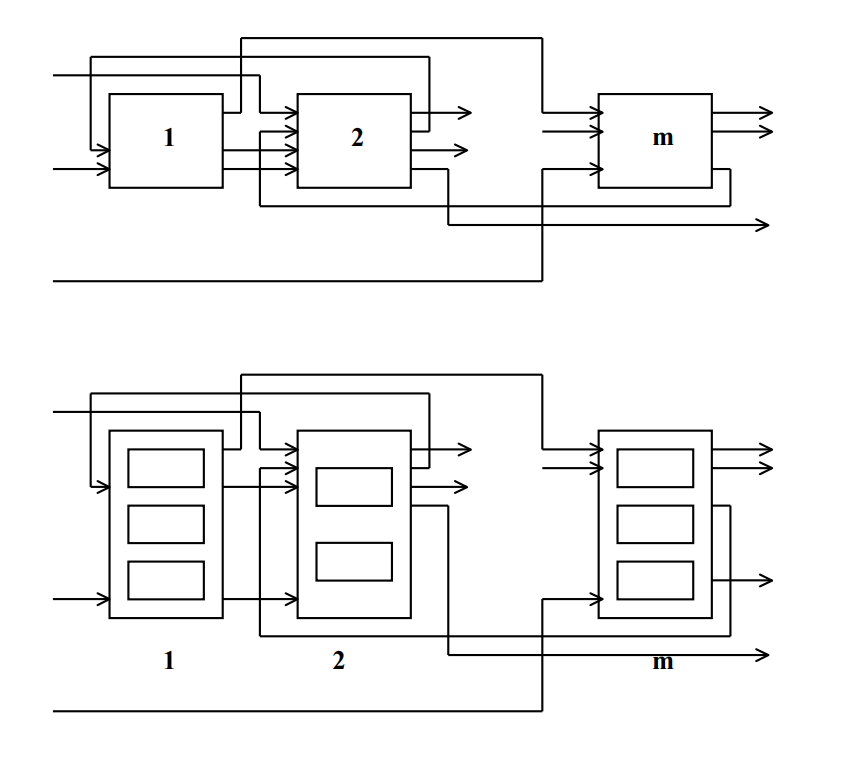
\includegraphics[scale = 0.5]{Rysunki/szeregowanie2.png}
\caption{Struktury gniazdowych systemów produkcyjnych: dedykowany (J), z maszynami równoległymi w stanowisku (PJ).}
\end{center}
\end{figure}

\begin{figure}[H]
\begin{center}
\label{diagram}
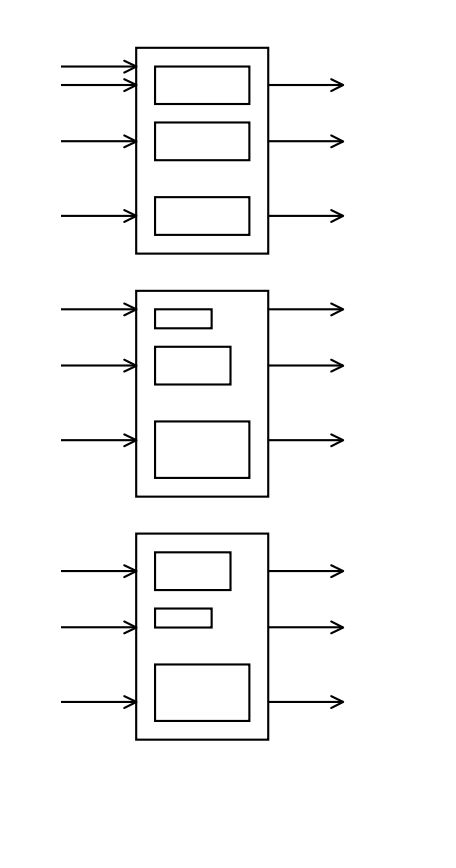
\includegraphics[scale = 0.5]{Rysunki/szeregowanie3.png}
\caption{ Struktury równoległych systemów produkcyjnych: maszyny
identyczne (P), jednorodne (Q), niejednorodne (R)}
\end{center}
\end{figure}
\subsection{Charakterystyka rozwiązań}
\begin{itemize}
\item Uszeregowanie częściowo aktywne --- gdy dla każdej operacji j z uszeregowania nie można jej ukończyć wcześniej przy:
\begin{itemize}
\item niezmienionym zbiorze maszyn,
\item każdorazowym identycznym czasie wykonywania wszystkich operacji innych niż j,
\item niezmienionej kolejności wykonywania operacji na każdej z maszyn.
\end{itemize}
\item Uszeregowanie aktywne ---  gdy dla każdej operacji j z uszeregowania nie można jej ukończyć wcześniej przy:
\begin{itemize}
\item niezmienionym zbiorze maszyn,
\item każdorazowym identycznym czasie wykonywania wszystkich operacji innych niż j,
\item niezmienionej kolejności wykonywania operacji innych niż j na każdej z maszyn,.
\end{itemize}
\item Uszeregowanie silnie aktywne --- gdy dla każdej operacji j z uszeregowania nie można jej ukończyć wcześniej przy:
\begin{itemize}
\item niezmienionym zbiorze maszyn przy wykonywaniu operacji innych niż j,
\item każdorazowym identycznym czasie wykonywania wszystkich operacji innych niż j,
\item niezmienionej kolejności wykonywania operacji innych niż j na każdej z maszyn.
\end{itemize}
\item Uszeregowanie lewostronnie optymalne ---  gdy dla każdej operacji j z uszeregowania nie można jej ukończyć wcześniej przy:
\begin{itemize}
\item każdorazowym identycznym czasie wykonywania wszystkich operacji innych niż j.
\end{itemize}	
\item Uszeregowanie nieopóźnione --- niezwłocznie rozpoczyna się wykonywanie operacji w sytuacji, gdy są one gotowe do wykonania oraz są wolne środki zasobowe do ich wykonania.
\item Uszeregowanie (K, S) "słabo nieopóźnione" (nieopóźnione) jeśli nie istnieje uszeregowanie (K, S'):
\begin{itemize}
\item zawierające operację j, której moment rozpoczęcia S'(j) jest wcześniejszy niż uprzednio (S(j)),
\item gdzie wszystkie maszyny z tego samego zbioru są wolne w chwili S'(j).
\end{itemize}
\item Uszeregowanie (K, S) "silnie nieopóźnione" jeśli nie istnieje uszeregowanie (K', S'):
\begin{itemize}
\item zawierające operację j , której moment rozpoczęcia S'(j) jest wcześniejszy niż uprzednio (S(j)),
\item $K'(i) \neq K(i), i \neq j$,
\item gdzie wszystkie maszyny z nowego zbioru K'(j) są wolne w chwili S'(j).
\end{itemize}
\end{itemize}






\newpage
\section{Strategie wytwarzania. Systemy sterowania}
\subsection{Strategia PUSH. Systemy MRP i ERP}
Strategia PUSH zakłada, że żądania wytwórcze (zamówienia na produkt końcowy) zostały przetłumaczone na żądania materiałów i półproduktów w określonych punktach wewnętrznych i na wejściach systemu dając szczegółowy bilans żądań materiałowych (MRP, Material Requirements Planning). Materiały dostarczone na wejście systemu są następnie przepychane (PUSH) za pomoca sterowań stopniowo w kierunku wyjścia systemu według ustalonego harmonogramu działań (schedule), określającego dla każdej zaplanowanej czynności termin rozpoczęcia i zakończenia oraz zbiór zasobów przydzielonych do jej realizacji. Podstawowy system MRP nie rozdziela ograniczonych zasobów (personel i maszyny) do realizacji zadań, lecz dostarcza jedynie statystyki ich dostępności i zapotrzebowań, pozostawiając podjęcie decyzji człowiekowi, który ostatecznie jest współtwórcą końcowego harmonogramu pracy systemu. Alternatywnie rozdziału takiego dostarcza system zarządzania zasobami produkcyjnymi przedsiębiorstwa (MRP II, Manufacturing Resource Planning), którego wynikiem jest nadrzędny harmonogram pracy systemu wytwarzania (master schedule), bilansujący możliwości wykonawcze i zamówienia. Podobne cechy ma bardziej zaawansowany system dystrybuujący wszystkie zasoby przedsiębiorstwa (ERP, Enterprise Resource Planning, nazywany także czasami MRP III). Realizacja harmonogramu nadrzędnego jest monitorowana. W razie potrzeby harmonogram jest korygowany i odpowiednie sterowania są przekazywane do systemu wytwarzania, w celu uzyskania zgodności stanu systemu i wyjść z programowo założonym stanem i programową wartością wyjść. Sterowanie tego typu nosi nazwę sterowania nadążnego. Strategie MRP, MRP II, ERP są polecane dla produkcji jednostkowej i krótkoseryjnej, przy wykorzystaniu pojedynczych maszyn w konwencjonalnych systemach wytwarzania oraz w pełni zautomatyzowanych elastycznych systemach wytwarzania (FMS, Flexible Manufacturing Systems). Systemy sterowania oparte na strategii PUSH są systemami zcentralizowanymi (jednopoziomowymi) lub hierarchicznymi wielopoziomowymi ze zwrotnym sprzężeniem informacyjnym pomiędzy poziomami. Monitorowaniu podlegają wszystkie stanowiska wytwarzania. Systemy PUSH mogą być z powodzeniem modelowane i analizowane w kategoriach klasycznej teorii szeregowania zadań i rozdziału zasobów.

\subsection{Strategia SQUEZEE. Systemy OPT}
Strategia SQUEZEE zakłada, że wydajność systemu wytwórczego jest ograniczona przepustowością wąskiego przekroju (nazywanego także wąskim gardłem) systemu. Przekrój ten jest zestawem stanowisk wytwórczych, przez które produkcja się przeciska (SQUEZEE) powodując spiętrzenia i kolejki zadań. Zwiększenie wydajności systemu poprzez wzrost mocy przerobowej stanowisk (wymiana urządzeń lub rozszerzenie liczby realizatorów) jest oczywisty i nie będzie tutaj dyskutowany. Zajmiemy się wyłącznie sterowaniem przepływu zadań przez wąskie gardło. Strategia OPT ustala optymalnie harmonogram pracy stanowisk wąskiego przekroju, a następnie dostosowuje harmonogram pracy pozostałych stanowisk w celu uzyskania kompletnego rozwiązania dopuszczalnego. Celem nadrzędnym jest optymalne wykorzystanie stanowisk krytycznych lub terminowość przejścia zadań przez cały system. Strategia OPT nadaje~się dobrze dla produkcji krótko- i średnio-seryjnej technologicznie zorientowanej, w realizacji zleceń niewrażliwych na zmiany terminów realizacji (w tym terminu zakończenia), w przypadku niewielkiej liczby stanowisk wąskiego przekroju (jedno wąskie gardło). %Systemy sterowania oparte na strategii SQUEZEE są systemami scentralizowanymi (jednopoziomowymi) lub hierarchicznymi wielopoziomowymi ze~zwrotnym sprzężeniem informacyjnym pomiędzy poziomami. W czasie pracy systemu tylko stanowiska krytyczne są monitorowane w celu korygowania bieżącego harmonogramu. Systemy SQUEZEE mogą być z powodzeniem modelowane i analizowane w kategoriach klasycznej teorii szeregowania zadań, niekiedy przy~rozszerzonych klasach funkcji kryterialnych.

\newpage
\subsection{Strategia PULL. Systemy JIT (Just-in-Time)}
Filozofię wytwarzania dokładnie na czas (JIT, Just in Time) stworzyli w znacznej mierze Japończycy. Pierwsze opisane
przypadki pochodziły z linii montażowej Toyoty. Strategia ta przyjmuje za~podstawę produkcji zgłoszoną wielkość zapotrzebowania na określony produkt finalny, który powoduje powstanie ssania (PULL) na wyjściu systemu wytwarzania. Ssanie to jest następnie tłumaczone na ssanie materiałów i półproduktów, skierowanych pod adresem stanowisk poprzednich i rozprzestrzenia się od wyjścia systemu przeciwprądowo w kierunku wejścia systemu. Brak ssania oznacza bezczynność systemu i stanowisk wytwarzania, zapobiegając zbędnemu wytwarzaniu produktu na zapas. Stworzone w ten sposób informacyjne sprzężenie zwrotne pozwala na samosterowanie się systemu i jego adaptację do żądań zgłoszonych na~wyjściu. Faktycznie “czysta” strategia zakłada, że nie ma żadnych zewnętrznych zmiennych sterujących, zaś sterowania lokalne są wyznaczane jednoznacznie poprzez odpowiednie sprzężenia zwrotne. Celem systemu jest możliwie szybka adaptacja aktualnego wyjścia do wyjścia zadanego, przy~czym wszystkie wielkości mają charakter dynamiczny. System JIT nie akumuluje (ZI, zero inventory) lub minimalizuje akumulację półproduktów w poszczególnych stadiach procesu poprzez dostarczanie produktów “na żądanie” i dokładnie-na-czas. W konsekwencji pozwala to ograniczyć zarówno powierzchnię produkcyjną, jak i zamrożone środki kapitałowe odpowiadające produkcji w toku oraz zwiększyć płynność przepływu produkcji. Stąd często w systemach tego typu pojawiają się żądania przepływu bez czekania (no wait), baz składowania (no store), z ograniczonym składowaniem (limited store) oraz nieregularne funkcje kryterialne, żądające wykonania dostawy w ściśle określonym przedziale czasu. Jednakże w celu uzyskania perfekcyjnego funkcjonowania takiego systemu potrzeba spełnić pewne dodatkowe warunki o charakterze organizacyjnym, a mianowicie: (a) niezawodne wejście do systemu materiałów i półproduktów na każde żądanie, (b) precyzyjna kontrola jakości na poszczególnych stanowiskach połączona z~wysoką jakością wytwarzanego produktu, (c) niezawodność środków wytwarzania (sprzęt, personel). Tak sformułowane wymagania rodzą dalsze działania o charakterze organizacyjnym jak np. rygorystyczna i planowana konserwacja zapobiegawcza maszyn, wiarygodność poddostawców, stabilność dostaw, fachowość pracowników, szerokie wielofunkcyjne wyszkolenie pracowników, itp. W~wielu systemach JIT przyjmuje się, że~przepływ zadań produkcyjnych odbywa się na zamówienie nie pojedynczo, lecz małymi porcjami. Technika ta zwana Kanban powszechnie uważana jest za integralny element systemów JIT. Żądanie (ssania) na materiały lub półprodukty wewnątrz systemu ma postać karty zamówienia o określonej wielkości partii (Kanban), przesyłanej cyklicznie między kooperującymi stanowiskami. Liczba krążących kart, jak~i~wielkość zamówienia jest ustalana arbitralnie przez nadrzędny system sterowania. W konsekwencji pomiędzy poszczególnymi stadiami procesu produkcyjnego pojawiają się ściśle kontrolowane, niewielkie zapasy, które pozwalają m.in. na wygładzanie naturalnych fluktuacji procesu, zapewnienie ciągłej realizacji zamówień, szybkie reagowanie na zgłoszone zamówienia. Strategia JIT dobrze nadaje się dla systemów wyposażonych w linie produkcyjne i gniazda wytwórcze z produkcją średnio-, wielkoseryjną i masową. Systemy sterowania oparte na strategii PULL są stosunkowo proste i rozproszone. Funkcje lokalnego sterowania ze sprzężeniem zwrotnym na najniższym poziomie spełniają karty Kanban. Parametry pracy tak określonego sterownika lokalnego (liczb kart, wielkość partii) mogą być ustalone przez planistyczno-sterujący człon nadrzędny, choć w praktyce po osiągnięciu stanu ustalonego procesu taka ingerencja jest rzadka. Systemy PULL wykraczają poza ramy klasycznej teorii szeregowania zadań, ze~względu na nietypowe ograniczenia i postacie funkcji kryterialnych. Dość często analizowane są poprzez modele przepływu, zaś ze względu na charakter opisu, badane narzędziami symulacyjnymi.

\subsection {Strategia CAW (Constant Average Workload)}
Strategia CAW steruje zleceniami produkcyjnymi w celu zapewnienia stałego średniego obciążenia stanowisk. Wspomaga ona MRP II w produkcji seryjnej. Jest polecana gdy terminy dostaw są stałe, zdolności produkcyjne są niezmienne, realizacja zadań na stanowiskach jest monitorowana, dostawy materiałów są stabilne.
\subsection {Strategia CRS (Continuous Replenishment of Stocks)}
Strategia CRS dąży do ciągłego uzupełniania bilansowanych stanów potrzeb materiałowych. Jest polecana dla produkcji, w przeważającej części seryjnej i powtarzalnej, płynnej, ze stałym zapotrzebowaniem materiałów niezależnie od długości serii, monitorowanej.





\newpage
\section{Problem pakowania. Sformułowanie, własności i metoda rozwiązywania}
\subsection{Sformułowanie problemu}
Danych jest n obiektów, każdy o pewnym rozmiarze $w_{i}$. Dana jest też dowolnie duża liczba skrzyń, z~których każda ma ustaloną pojemność W. \\
\textbf{Problem pakowania pudełek} --- (ang. Bin Packing Problem - BPP) należy do
dużej rodziny zagadnień grupowania elementów, które polegają na podziale
zbioru elementów na rozdzielne podzbiory. Problemy~te należą do NP-trudnych
problemów optymalizacji kombinatorycznej. BPP formułujemy następująco:
mamy n niepodzielnych obiektów, każdy o wadze (wartości) $w_{i}$, (1in) oraz n pudełek (ang. bins) każde o pojemności C ($w_{i}$<C); należy tak rozmieścić obiekty w pudełkach, by liczba użytych pudełek była minimalna, przy założeniu, że pojemność pudełek nie będzie przekroczona.

\subsection{Własności}
\begin{itemize}
\item Problem jest NP-trudny.
\item Najgorszy przypadek --- użytych pudełek tyle, ile przedmiotów do włożenia (po 1 na pudełko).
\item Dolne ograniczenie (najlepszy wynik): Wszystkie pudełka zapakowane po brzegi:
$z = \sum_{i=1}^{n} \frac{w_{i}}{c})$.
\end{itemize}

\subsection{Metody rozwiązywania}
\indent Proste algorytmy rozwiązujące w sposób przybliżony problem pakowania
pudełek podali Garey i~Johnson; spośród nich \textbf{algorytm First Fit Decreasing
(FFD)}, daje w wyniku rozwiązanie nie gorsze niż~22\% od rozwiązania
optymalnego. W 1990 roku Martello i Toth zaproponowali \textbf{algorytm przeglądu z~nawrotami}, osiągając bardzo dobre rezultaty. W ostatnim okresie trwają intensywne prace nad zastosowaniem \textbf{algorytmów ewolucyjnych do różnych problemów optymalizacji kombinatorycznej.} W przypadku BPP pojawił się specjalizowany algorytm
genetyczny Falkenauera GGA bazujący na specjalizowanej reprezentacji
problemu oraz specjalnie skonstruowanych operatorach pseudogenetycznych.\\
\indent Problem ten jest NP-trudny, ale dość dobrze aproksymowalny.
Istnieje prosty, choć dosyć skuteczny \textbf{algorytm zachłanny: sortujemy obiekty malejąco, po czym w tej kolejności próbujemy umieszczać je w kolejnych skrzyniach. Ostatecznie umieszczamy obiekt w pierwszej skrzyni, w której się zmieści.}





\newpage
\section{Problem komiwojażera. Sformułowanie, własności i metoda rozwiązywania}
\subsection{Sformułowanie problemu}
\noindent \textbf{Problem komiwojażera} --- (TSP -- ang. travelling salesman problem) jest to zagadnienie optymalizacyjne, polegające na znalezieniu minimalnego cyklu Hamiltona w pełnym grafie ważonym (drogi mają wagi).\\
Nazwa pochodzi od typowej ilustracji problemu, przedstawiającej go z punktu widzenia wędrownego sprzedawcy (komiwojażera): dane jest n miast, które komiwojażer ma odwiedzić (każde miasto tylko raz), oraz odległość/cena podróży/czas podróży pomiędzy każdą parą miast. Celem jest znalezienie najkrótszej/najtańszej/najszybszej drogi łączącej wszystkie miasta zaczynającej się i kończącej się w określonym punkcie.
Symetryczny problem komiwojażera (STSP) polega na tym, że dla dowolnych miast A i B odległość z A do B jest taka sama jak z B do A. W asymetrycznym problemie komiwojażera (ATSP) odległości te mogą być różne.\\
Rozwinięciem problemu komiwojażera jest problem marszrutyzacji.
Cykl Hamiltona to taki cykl w grafie,

\subsection{Własności}
\begin{itemize}
\item Silnie NP-trudny,
\item cykli w grafie o n wierzchołkach jest $(n!)/2$.
\end{itemize}

\subsection{Metody rozwiązywania}
\begin{itemize}
\item Algorytm NEH,
\item bruteforce tylko dla małych n, około 10,
\item najpopularniejsze metody podziału z modyfikacjami, branch-and-bound, branch-and-cut,
\item najbliższy sąsiad, sprawdź dystanse do pozostałych, wybierz najmniejszy. Wynik zależy od wierzchołka, z którego startujemy.
\end{itemize}



\newpage
\section{Problem plecaka. Sformułowanie, własności i metoda rozwiązywania}
\subsection{Sformułowanie problemu}
\noindent \textbf{Dyskretny problem plecakowy} --- (ang. discrete knapsack problem) jest jednym z najczęściej poruszanych problemów optymalizacyjnych. Nazwa zagadnienia pochodzi od maksymalizacyjnego problemu wyboru przedmiotów tak, by ich sumaryczna wartość była jak największa i jednocześnie mieściły się w~plecaku. Przy podanym zbiorze elementów o podanej wadze i wartości, należy wybrać taki podzbiór, by~suma wartości była możliwie jak największa, a suma wag była nie większa od danej pojemności plecaka. Problem plecakowy często przedstawia się jako problem złodzieja rabującego sklep – znalazł on N~towarów; j–ty przedmiot jest wart $c_{j}$ oraz waży $\omega_{j}$ . Złodziej dąży do zabrania ze sobą jak najwartościowszego łupu, przy czym nie może zabrać więcej niż B kilogramów. Nie może też zabierać ułamkowej części przedmiotów (byłoby to możliwe w ciągłym problemie plecakowym).

\subsection{Metody rozwiązywania}
\subsubsection{Przegląd zupełny}
Przegląd zupełny (bruteforce, metoda siłowa) --– metoda nieefektywna obliczeniowo (ale jak najbardziej optymalna, gdyż znajduje rozwiązanie najlepsze); w jego przypadku złożoność obliczeniowa algorytmu wyniesie $\Theta(2^{n})$, co zdecydowanie zawyży czas działania dla dużych n. Złożoność wynosi $\Theta(2^{n})$, ponieważ jest tyle możliwych ciągów zero jedynkowych na n polach. Złożoność można również obliczyć ze wzoru dwumianowego Newtona (dwumian Newtona), podstawiając za a i b jedynki.

\textbf{Własności:}
\begin{itemize}
\item jest NP-trudny (sprawdzenie pojedynczego rozwiązania ma wielomianową złożoność obliczeniową),
\item nie znamy algorytmu wielomianowego.

\end{itemize}

\subsubsection{Rozwiązania dynamiczne}
Programowanie dynamiczne z zapisywaniem obliczonych wartości do tablicy T(n, m), gdzie  m to~liczba zapakowanych przedmiotów. Rozwiązanie znajduje się w komórce T (n, m). 
\subsubsection{Algorytm aproksymacyjny}
W pierwszej części algorytmu zachłannego przedmioty są sortowane według stosunku wartości do wagi (po lewej), po czym wybierane są kolejno od góry te elementy, które się jeszcze mieszczą w plecaku.\\
\indent W wersji zachłannej algorytm aproksymacyjny sortuje elementy w kolejności malejącej, porównując stosunek wartości do wagi elementu. Następnie wstawia je kolejno, zaczynając od przedmiotu o największym ilorazie do plecaka. Jeśli jakiś element nie mieści się w plecaku, to jest omijany, a algorytm przechodzi do następnego. W algorytmie wybierany jest maksymalny wynik z tak obliczonego upakowania plecaka oraz plecaka z elementem o największej wartości. Jeśli k jest maksymalną wartością przedmiotów w optymalnie upakowanym plecaku, algorytm zachłanny osiąga wyniki nie gorsze niż k/2. Złożoność obliczeniowa algorytmu zależy od sortowania $\Theta(n\log(n))$.

\newpage
\section{Optymalizacja pracy jednomaszynowego stanowiska krytycznego. Sformułowanie,
właściwości i metoda rozwiązywania}
\subsection{Sformułowanie problemu}
\indent Stanowisko krytyczne to takie, które posiada ograniczenia przepustowości. Dla jednomaszynowego stanowiska krytycznego problem optymalizacji polega na znalezieniu takiego uszeregowania zadań, dla~którego czas wykonania całości będzie najmniejszy.\\
\textbf{Problem podstawowy}\\
\indent Załóżmy, że zbiór zadań $J=\{1,2,...,n\}$ ma być wykonywany na jednej maszynie o ograniczonej jednostkowej przepustowości $(1<=k<\infty)$. Każde zadanie składa się z pojedynczej operacji posiadającej ustalony, znany a priori, czas wykonywania $P_{j}$>0, 1<=j<=n. Rozwiązaniem jest harmonogram pracy stanowiska reprezentowany przez wektory terminów rozpoczęcia $S=(S_{1},...,S_{n})$ oraz zakończenia zadań $C=(C1,...,Cn)$, spełniające powyższe ograniczenia. W praktyce, ponieważ $C_{j}=S_{j}+P_j$, zatem rozwiązanie jest całkowicie charakteryzowane przez jeden z tych wektorów. Jeśli funkcja celu jest regularna, to harmonogram optymalny leży w klasie harmonogramów dosuniętych w lewo. Wtedy~też każdy harmonogram może być jednoznacznie reprezentowany kolejnością wykonywania zadań na stanowisku, ta z kolei jest reprezentowana permutacją 
$\pi =(\pi(1),...,\pi(n))$ na zbiorze J. W tym przypadku dla danej permutacji $\pi$ terminy rozpoczęcia $S_{j}=C_{j}-P_{j}$ i zakończenia wykonywania $C_{j}$ określone są wzorem:
$C_{\pi(j)}=C_{\pi(j-1)} + P_{\pi(j)}, j=1,...,n$
gdzie $\pi(0)=0$ oraz $C_{0}=0.$ Jeśli funkcją kryterialną jest $C_{max}$, to~każda permutacja jest optymalna.\\\\
\indent W zależności od sformułowanych potrzeb, optymalizować można różne kryteria. Do najbardziej popularnych należą: czas przepływu wszystkich produktów przez stanowisko, średni czas przepływu obiektu przez stanowisko, czas wyjścia ostatniego produktu ze stanowiska.
\subsection{Właściwości}
\noindent \textbf{Silnie NP-trudny}\\
\subsection{Metody rozwiązywania}
\begin{itemize}
\item FIFO, FCFS O(logr)
\item Schrage
\item Schematy aproksymacyjne
\end{itemize}




\newpage
\section{Optymalizacja pracy linii wytwórczej. Sformułowanie, właściwości i metoda rozwiązywania}
\subsection{Sformułowanie problemu}
Dany jest zbiór $Z = \{1,2, ... ,n\}$ n zadań do wykonania przez m maszyn. Liczba zadań n oraz liczba maszyn m są znane i określone jako parametry wejściowe problemu. Każde zadanie $z \in Z$ jest określone przez m czasów wykonania dla każdej maszyny. Będą to czasy kolejno $t_{1j},t_{2j}, ..., t_{mj}$ dla każdej z m~maszyn. Wszystkie zadania wykonywane są przez każdą z maszyn w kolejności <1,2,..., m>. Rozpoczęcie zadania j na maszynie i nie może się zacząć wcześniej, niż zostanie ono zakończone na maszynie i-1.\\
\noindent \textbf{Założenie}\\
 Przyjęto, że kolejność wykonywania zadań przez każdą z maszyn jest taka sama. Założenie jest również takie, że nie można przerwać wykonywania zadania w dowolnym momencie, czyli nie istnienie pojęcie wywłaszczania zadań z maszyny.
 
\subsection{Właściwości}
\begin{itemize}
\item Gdy liczba maszyn m = 2 algorytm jest rozwiązywalny w czasie wielomianowym. 
\item Dla m większej niż 2 problem jest silnie NP-trudny.
\end{itemize}

\subsection{Metody rozwiązywania}
Oznaczmy przez $C_{ij}$ moment zakończenia wykonywania zadania j przez maszynę i. Wówczas problem polega na znalezieniu takiej kolejności wykonywania zadań, która minimalizuje długość szeregowania $C_{max} = max( j \in J\{C_{mn}\})$.

\subsubsection{Algorytm NEH}
Nazwa algorytmu pochodzi od pierwszych
liter nazwisk jego twórców: Nawaza, Enscore'a i Hama. NEH jest algorytmem
deterministycznym, czyli zawsze dającym te same wyniki dla danego zestawu
danych wejściowych.
 
Algorytm NEH polega na początkowym obliczeniu długości wykonywania się każdego zadania. Następnie zadania należy uporządkować w kolejności nierosnącej. Kolejno trzeba wsadzać zadania na każdej możliwe pozycji i wybrać to o najmniejszej wartości Cmax.
\subsubsection{Just-in-Time [JIT]} 
Można użyć japońskiego systemu JIT (Toyota). Powstał, by operacje miały miejsce dokładnie wtedy, gdy są potrzebne. Jeśli materiały przychodzą na czas, zapasy produkcji w toku mogą być wyeliminowane. Jedną z prostych realizacji koncepcji JIT jest system KANBAN.\\\\
Najkrócej ideę \textbf{KANBAN} oddaje hasło „7 x żadnych”:
\begin{itemize}
\item żadnych braków,
\item żadnych opóźnień,
\item żadnych zapasów,
\item żadnych kolejek – gdziekolwiek i po cokolwiek,
\item żadnych bezczynności,
\item żadnych zbędnych operacji technologicznych i kontrolnych,
\item żadnych przemieszczeń.
\end{itemize}



 


\newpage
\section{Optymalizacja pracy systemu opartego na przetwarzaniu różnych zadań. Sformułowanie, właściwości i metoda rozwiązywania}
\noindent \textbf{Problem Job shop}\\
\indent Problem Job shop polega na szeregowaniu zadań dla zleceń jednostkowych o ustalonych liniowych marszrutach. Każde zlecenie składa się z zadań wykonywanych na osobnych maszynach, ustawionych w określonej kolejności, z konkretnymi czasami ich przetwarzania na danej maszynie.
W problemie Job shop, w przypadku gdy więcej niż jedno zadanie oczekuje przed maszyną na wykonanie, wtedy mamy do czynienia z konfliktami na maszynach. Jest to związane z tym, że każda maszyna może wykonywać tylko jedną operację w danej chwili i żadna operacja nie może być jednocześnie wykonywana przez różne maszyny (zasada wzajemnego wykluczania przydziału maszyn do operacji). Do rozwiązania takiego problemu stosujemy jedną z wielu znanych w literaturze reguł priorytetu.
\\\\
\textbf{Najczęściej stosowane są następujące reguły priorytetu:}
\begin{itemize}
\item FIFO - zadanie, które weszło na maszynę jako pierwsze, w przypadku konfliktu wykonywane jest jako pierwsze.
\item SPT - (ang. shortest processing time), czyli wybieramy to zadanie, które ma najkrótszy czas przetwarzania.
\item EDD - (ang. earliest due date), liczymy sumę czasów począwszy od przybycia zlecenia do systemu, aż do zakończenia danego zlecenia i wybieramy zlecenie z mniejszą sumą.
\item LIFO - zadanie, które weszło na maszynę jako ostatnie, w przypadku konfliktu, wykonywane jest jako pierwsze.
\item LPT - (ang. latest processing time), czyli wybieramy to zadanie, które ma najdłuższy czas przetwarzania.
\item LWR - (ang. least work remaining), czyli w danym zleceniu liczymy sumę czasów pozostałych zadań potrzebnych do wykonania całego zlecenia i wybieramy to z sumą mniejszą.
\end{itemize}


\newpage
\section{Optymalizacja transportu. Przykładowy problem i metoda rozwiązywania}
\subsection{Sformułowanie problemu}
Transport jest dość specyficzną i trudną z organizacyjnego punktu widzenia działalnością. Między podejmowanymi decyzjami a efektywnością procesów transportowych istnieją nieliniowe zależności, które trudno jest przedstawić za pomocą matematycznych modeli. Generalnie problem optymalizacji transportu można określić w następujący sposób: należy opracować optymalny plan transportowy połączeń określonej liczby odbiorców od określonej liczby dostawców. Zakłada się, że są to jednorodne ładunki, a więc odbiorcy nie są
ograniczeni do na przykład jednego dostawcy, ale mogą wybierać spośród wszystkich dostępnych. Optymalizacja przewozów służy do takiego rozplanowania przewozów, aby~koszty transportu były jak najniższe. Dotyczy to głównie przedsiębiorstw, których działalność wymaga dokonywania transportu dużej ilości produktów np: zboża, węgla, piasku czy cementu.\\\\
\subsection{Metody rozwiązywania}

\textbf{Przykładowy problem II:}\\
Trzy magazyny: M1, M2, M3, zaopatrują w mąkę cztery piekarnie: P1, P2, P3, P4.
Należy opracować plan przewozu mąki z magazynów do piekarń, minimalizujący całkowite koszty transportu.

\begin{itemize}
\item metoda kąta północno-zachodniego,
\item metoda minimalnego elementu wiersza lub kolumny macierzy kosztów,
\item metoda minimalnego elementu macierzy kosztów.
\end{itemize}

\noindent \textbf{Rozwiązanie}
\begin{enumerate}
\item Znalezienie rozwiązania dopuszczalnego jedną z metod: pn.-zach. kąta, najmniejszego elementu, VAM.
\item Obliczenie kosztu rozwiązania.
\item Sprawdzenie, czy rozwiązanie jest zdegenerowane (czy jest odpowiednia ilość baz).
\item Jeżeli jest niezdegenerowane należy zastosować metodę e-perturbacji.
\item Sprawdzenie, czy rozwiązanie jest optymalne metodą potencjałów.
\item Jeżeli nie jest optymalne, należy stworzyć cykl i zbudować nowe rozwiązanie dopuszczalne.
\item Powtarzanie kroków 5 i 6 do momentu otrzymania rozwiązania optymalnego.
\end{enumerate}
\textbf{Rozwiązanie dopuszczalne} --- rozwiązanie, które w wyniku daje niski koszt ale jest możliwość w~prosty sposób uzyskania kosztu niższego. Jest to rozwiązanie przejściowe. Istnieje wiele rozwiązań dopuszczalnych dla jednego zagadnienia transportowego, przy czym każde kolejne ma lepszy (niższy) lub przynajmniej nie gorszy koszt od poprzedniego.
\\
\textbf{Rozwiązanie optymalne} --- rozwiązanie, które w wyniku daje koszt najniższy do uzyskania poprzez znane nam metody. Jest to rozwiązanie końcowe. Może istnieć kilka rozwiązań optymalnych dla jednego zagadnienia transportowego, lecz koszt każdego z nich powinien być taki sam. 




\newpage
\section{Balansowanie linii montażowej. Przykładowy problem i metoda rozwiązywania. Związek z szeregowaniem}
\noindent \textbf{Balansowanie linii montażowej} --- idea balansowania linii montażowej polega na wyznaczeniu minimalnej liczby stanowisk pracy (stacji, maszyn) poprzez optymalne, ale uwzględniające ograniczenia kolejnościowe, rozdzielenie operacji na stanowiska.\\
\textbf{Stacja robocza} jest to segment linii montażowej, na której wykonywane są określone operacje.\\
Zbiór wykonywanych operacji na stacji roboczej nazwano jej \textbf{obciążeniem}. Ruch na linii montażowej -> od początku do końca, bez pomijania stacji pośredniej.\\
\textbf{Operacja} jest to elementarna czynność całkowitego procesu montażu wykonywana na linii technologicznej. Czas konieczny do realizacji operacji nazwany został czasem wykonania operacji. Operacja jest rozważana jako czynność niepodzielna, gdyż żadna
z operacji nie może być podzielona ma mniejszą czynność.\\
\textbf{Założenia}
\begin{itemize}
\item Wszystkie parametry wejściowe są znane,
\item operacja nie może być przydzielona pomiędzy dwie lub
więcej stacji roboczych,
\item operacje muszą być wykonane zgodnie z wymaganiami
technologicznymi przedstawionymi w postaci relacji kolejnościowych,
\item wszystkie operacje muszą być wykonane,
\item czas wykonania operacji jest stały niezależnie od
przydzielenia do stacji roboczej,
\item linia nie posiada żadnych struktur równoległych
i jest rozważana jako szeregowa.
\end{itemize}
\textbf{Typy optymalizacji}
\begin{itemize}
\item Typ 1 --- cykl jest stały i dany.
Celem jest minimalizacja przestojów stacji, co jest równoważne z~minimalizacją
liczby stanowisk pracy.
\item Typ 2 --- liczba stacji jest dana i jest stała.
Celem jest minimalizacja cyklu balansowanej linii, co~jest
równoważne z maksymalizacją produkcji.
\end{itemize}


\noindent Optymalizując pracę linii wytwórczej chcemy uniknąć jakichkolwiek przestojów. Należy tak dobrać obciążenia na każdym odcinku, żeby praca na nich przebiegała w możliwie jak najbardziej równym tempie. Równoważenie obciążeń linii montażowej. Czyli, by czas wykonywania produktu najwolniejszego stanowiska był możliwie najszybszy. 
\\
\textbf{Przykładowy problem}\\
\indent Puszka coli najpierw jest formowana, potem napełniana, zamykana, na koniec pakowana do kartonów.\\
Każde z zadań odbywa się na innej stacji - w sumie 4.
Żeby przed żadnym z tych stanowisk nie tworzyły~się kolejki, można, np. rozdzielić ograniczoną liczbę pracowników/maszyn, żeby formowaniem puszki zajmowały się 72 osoby (bo to taka ciężka praca), a napełnianiem tylko 24. I żeby na pakowaniu była tylko 1~osoba, bo gdy pakujemy karton 24 puszkami, to pozostałe stanowiska powinny wyprodukować 24 puszki. Przykład z kategorii niepraktycznych :)
Dzięki temu linia jest zbalansowana, a produkcja zoptymalizowana.\\
\textbf{Sformułowanie zadania}\\
Tak rozdzielić zasoby, żeby wszyscy mieli po równo, żeby czas najdłużej pracującego stanowiska był mimo wszystko jak najkrótszy.
\begin{itemize}
\item Zbiór rozwiązań: $Z = max(T_i), i \in [1, m]$.
\item Rozwiązanie optymalne: $min(Z)$.
\end{itemize}
 
\noindent \textbf{Związek z szeregowaniem}\\
\indent Na jednej linii montażowej mogą być produkowane różne wersje produktu posiadające różne czasy na stanowiskach i dla takiego przypadku powinno się dodatkowo zastosować szeregowanie zadań, aby nie tworzyły się kolejki.

\noindent \textbf{Rozwiązanie}\\
Algorytmy BLM (heurystyczne):
\begin{itemize}
\item  Ranked positional wieght
\item  Kilbridge’a i Westera
\end{itemize}

\newpage
\section{Modele grafowe w badaniach operacyjnych. Przykładowy problem i metoda rozwiązywania}
\noindent\textbf{\href{https://fc.put.poznan.pl/sites/default/files/kkwarciak_rozprawa_streszczenie.pdf}{Może to?}} \\\\

\noindent \textbf{Problem:}\\
Graf składa się z wyróżnionych punktów zwanych węzłami grafu i odcinków łączących określone pary węzłów, zwanych  łukami grafu. Same modele grafowe pozwalają wyznaczyć metodę i rozwiązanie określonych problemów związanych z podjęciem optymalnych decyzji. 

Przykłady:
\begin{itemize}
\item produkcja filmu
\item budowa obwodnicy warszawy
\item prace organizacyjne 
%\item problem komiwojażera 
%\item problem plecakowy
%\item problem marszrutyzacji 
%\item jakikoliwiek problem
\end{itemize}

\noindent \textbf{Metoda rozwiązania:}\\
Całe przedsięwzięcie daje się rozłożyć na elementy prostsze zwane czynnościami. Każda czynność jest procesem wykonywania określonej części zadania stanowiącego wynik realizacji danego przedsięwzięcia. Czynność zaznacza się na wykresie w postaci strzałek (zwanych także łukami). Każda czynność trwa przez pewien czas t zwany czasem trwania. 

\begin{itemize}
\item \textbf{Metoda ścieżki krytycznej CPM (Critical Path Method)} - w każdym elemencie grafu wyznaczona jest wartość, dzięki którym czasy rozpoczęcia zadań dobierane są w taki sposób aby czas trwania całego projektu nie został wydłużony (czas poniżej którego nie można zejść - ścieżka krytyczna):
\begin{itemize}
\item \textbf{ES} - najszybszy czas rozpoczęcia 
\item \textbf{EF} - najszybszy czas zakończenia
\item \textbf{LF} - najpóźniejszy czas zakończenia
\item \textbf{LS} - najpóźniejszy czas rozpoczęcia 
\end{itemize}

\item \textbf{metoda PERT} - podobnie jak w przypadku metody CMP istotą metody PERT jest analiza ścieżki krytycznej. Różnica pomiędzy obiema metodami polega na traktowaniu w metodzie PERT czasu trwania zadania jako zmienną losową, nie natomiast jako zmienną zdeterminowaną, jak w przypadku CMP.
\end{itemize}



\newpage
\section{Modelowanie procesów dyskretnych: sieci Petri, DDES, systemy kolejkowe, symulacje}

\subsection{Sieci Petri}
\textbf{Sieć Petriego} –- matematyczna reprezentacja dyskretnych systemów rozproszonych. Sieci Petriego zostały zdefiniowane w latach 60. XX w. przez Carla Adama Petriego. Przez swoją zdolność do~wyrażania współbieżnych zdarzeń uogólniają one teorię automatów.\\

Sieć Petriego w najprostszej wersji składa się z "miejsc", "tranzycji"\ oraz krawędzi skierowanych. Taką siecią można jedynie opisać układ jako statyczne połączenie możliwych do osiągnięcia stanów. Aby~opisać konkretny stan układu, potrzebne są "żetony", które można przemieszczać pomiędzy miejscami poprzez przejścia po krawędziach grafu. Tradycyjnie miejsce oznacza się okręgiem, w którym można umieścić żeton prezentowany przez koło. W jednym miejscu może znajdować się dowolna, nieujemna liczba żetonów. Tranzycje oznacza się prostokątami lub kreskami, a krawędzie to strzałki. Krawędzie mogą mieć wagi większe lub równe 1. Wagi równej 1 nie oznacza się, tak jak pokazano na~rysunku. Waga określa, ile dokładnie żetonów przechodzi po krawędzi.
\begin{figure}[H]
\begin{center}
\label{diagram}
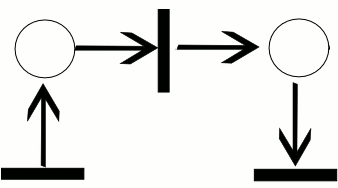
\includegraphics[scale = 1]{Rysunki/Petri.png}
\caption{Petri - Wiki}
\end{center}
\end{figure}

W najprostszej postaci żetony w sieci Petriego są nierozróżnialne między sobą. Bardziej złożone postacie sieci Petriego korzystają z pojęć kolorowania żetonów, czasu aktywacji przejść oraz hierarchii. Poza nimi istnieje wiele innych różnych rozszerzeń Sieci Petriego, takich jak sieci obiektowe (z żetonami, które mogą być Sieciami Petriego), z ograniczonymi pojemnościami miejsc, łukami wzbraniającymi i inne.\\




\subsection{DDES}
\noindent \textbf{Distributed discrete event simulations}\\
Tradycyjne dyskretne symulacje wyjątków implementują algorytm sekwencyjny. W praktyce symulacje dużych systemów są ograniczone przez właśnie ich sekwencyjność, ponieważ mała liczba wyjątków może być zasymulowana. Rozpowszechniona dyskretna symulacja wyjątków jest alternatywą i może doprowadzić do lepszej wydajności poprzez dzielenie symulacji pomiędzy procesory komponentów. Kilka technik jest zasugerowanych do detekcji oraz zapobieganiu zastoju.
\subsection{Systemy kolejkowe}
Zgłoszenia są jednorodne, ale przychodzą losowo. Odstęp pomiędzy zdarzeniami i zdarzenia przychodzą losowo. Czas rejestracji zgłoszenia jest znikomo mały, jest to proces Markowa --– przyszły proces zależy od bieżącego procesu a nie od procesów poprzednich. Nie ma znaczenia, ile procesów przyszło wcześniej.
\subsection{Symulacje}
Metody naukowe pozwalające na poszukiwanie optymalnych rozwiązań są rozwijane od wielu lat. Są~one m.in. przedmiotem tzw. badań operacyjnych, w ramach których powstało wiele metod analitycznych pozwalających na sprawne poszukiwanie optymalnych rozwiązań. Są to jednak metody mające wiele ograniczeń i rozwiązujące tylko określone problemy z różnych dziedzin. Ich zaletą jest możliwość znalezienia optymalnego rozwiązania, czyli najlepszego, w miarę prosty sposób. Jednak ze względu na~różnorodność problemów i stopień skomplikowania bardzo często nie można znaleźć gotowych metod analitycznych, które można wykorzystać do poszukiwania optymalnego rozwiązania. W tych przypadkach, w których rozwiązania nie możemy znaleźć za pomocą metod analitycznych, mogą być wykorzystane chociażby metody heurystyczne, a w przypadku optymalizacji, np. algorytmy ewolucyjne. W wielu przypadkach jedynym wyjściem jest jednak zastosowanie metod symulacyjnych.\\
\indent Charakterystyczną cechą metod symulacyjnych, wychodząc od znaczenia łacińskiego słowa simulatio, jest udawanie rzeczywistego zachowania się badanego obiektu lub systemu. Jako obiekt rozumiany jest wyodrębniony element z otaczającej nas rzeczywistości o charakterze materialnym lub abstrakcyjnym. Możemy mówić o różnych rodzajach obiektów, np.: fizycznych, technicznych, matematycznych itp.\\
Jako system rozumiany jest wyodrębniony z otoczenia zbiór obiektów powiązanych ze sobą odpowiednimi relacjami opisującymi wzajemne oddziaływanie obiektów na siebie. Wyróżniamy systemy występujące w naturalny sposób w otaczającej nas rzeczywistości oraz systemy zbudowane przez człowieka. Podstawą umożliwiającą przeprowadzenie symulacji jest zbudowanie modelu badanego obiektu lub systemu. Sama zaś symulacja polega na uproszczonym odtwarzaniu zachowania się obiektu lub systemu poprzez jego model. Najważniejszym wymaganiem stawianym modelom symulacyjnym jest konieczność poprawnego naśladowania zachowania się ich oryginalnych pierwowzorów. W praktyce spotyka się zasadniczo dwa rodzaje modeli symulacyjnych, czyli modele fizyczne lub matematyczne. Modele fizyczne są często pomniejszone w odpowiedniej skali w stosunku do oryginału. Modele matematyczne bardzo często są~zapisywane w postaci odpowiedniego programu komputerowego. W programie tym są zamodelowane najistotniejsze cechy systemu i jego oddziaływanie z otoczeniem. Badanie zachowania się modelu (modelowanego systemu) polega na zmianie odziaływania otoczenia na model w postaci sygnałów wejściowych i zmianie zachowania się samego systemu w wyniku zmiany jego parametrów.
W zależności od cech modeli symulacyjnych, które często wynikają bezpośrednio z cech modelowanych systemów, modele możemy podzielić na:
\begin{itemize}
\item dynamiczne – w których stan systemu ulega zmianie w z upływem czasu,
\item interaktywne – reagujące na sygnały zewnętrzne,
\item nieinteraktywne – odizolowane od otoczenia,
\item statyczne – w których czas nie ma wpływu na zmiany stanu systemu,
\item deterministyczne – w których nie występują zmienne o charakterze losowym,
\item stochastyczne – w których występują zmienne o charakterze losowym,
\item z czasem dyskretnym – w których upływ czasu jest dyskretyzowany ze stałym krokiem,
\item zdarzeń dyskretnych – w których czas podlega zmianom skokowym w zależności od zaistnienia zdarzeń dyskretnych.
\end{itemize}
Typ budowanego modelu symulacyjnego oraz poziom szczegółów, z jakim odzwierciedla on system rzeczywisty zależy w dużym stopniu od rodzaju symulowanego systemu oraz celu przeprowadzania symulacji. W ogólnym przypadku można dokonać podziału celów symulacji na dwie grupy. Pierwsza grupa obejmuje zastosowanie symulacji komputerowej do badania zachowania się systemów nieistniejących, które są w fazie projektowania. Druga grupa obejmuje symulacje zachowania się systemów istniejących,
których przeprowadzenie na systemie rzeczywistym jest niemożliwe lub bardzo kosztowne. Koszt eksperymentu symulacyjnego, ma decydujący wpływ na wybór stosowanej metody symulacyjnej, a często w ogóle decyduje o rozpoczęciu prac w tym zakresie. Budowanie komputerowych modeli symulacyjnych wymaga odpowiedniego przygotowania merytorycznego, doświadczenia w danym zakresie tematycznym i odpowiednich narzędzi. Samo zbudowanie modelu może być bardzo kosztowne ze względu na konieczność zebrania wielu informacji i danych oraz przeprowadzenia dokładnej analizy, w jakim stopniu informacje te są istotne dla budowanego modelu.\\
\indent Kolejnym etapem jest weryfikacja poprawności modelu symulacyjnego. Na tym etapie należy sprawdzić, czy zachowanie modelu symulacyjnego jest zgodne z zachowaniem systemu rzeczywistego. Bardzo często takie bezpośrednie porównanie jest niemożliwe, co bardzo utrudnia budowanie modeli symulacyjnych.\\
\indent Kolejny etap, czyli przeprowadzenie eksperymentu symulacyjnego może być długotrwałe i kosztowne, szczególnie w przypadku symulacji systemów bardzo złożonych, gdy celem jest optymalizacja, która wymaga przeprowadzenia wielu symulacji. Ponadto możliwość poszukiwania optymalnych rozwiązań w~oparciu o metody symulacyjne jest ograniczona. Wybór najlepszego rozwiązania może być dokonany tylko na podstawie przeprowadzonych eksperymentów symulacyjnych, których liczba jest ograniczona. Nie ma żadnych gwarancji, że kolejna symulacja z innymi parametrami nie dałaby lepszego rozwiązania.
Mimo opisanych powyżej trudności związanych z przygotowaniem i przeprowadzeniem eksperymentu symulacyjnego, metoda ta znajduje bardzo szerokie zastosowanie w wielu dziedzinach życia.



\newpage
\section{Programowanie liniowe. Sformułowanie, metody rozwiązywania, przykład zastosowania.}
\noindent\textbf{\href{http://tarapata.strefa.pl/p_ekonometria/download/ekonometria\%20_cz3_1a.pdf}{Dodatkowe przykłady 1}} \\
\textbf{\href{https://www.ksiegarnia.beck.pl/media/product_custom_files/1/1/11643-badania-operacyjne-z-wykorzytsaniem-winqsb-dariusz-siudak-darmowy-fragment.pdf}{Dodatkowe przykłady 2}} \\


Programowanie liniowe – klasa problemów programowania matematycznego, w której wszystkie warunki ograniczające oraz funkcja celu mają postać liniową. Warunki ograniczające mają postać:\\
$a_{1}x_{1} + a_{2}x_{2} + ... + a_{n}x_{n} \geq a$ \\
$a_{1}x_{1} + a_{2}x_{2} + ... + a_{n}x_{n} \leq a$ \\
$a_{1}x_{1} + a_{2}x_{2} + ... + a_{n}x_{n} = a$ \\

\noindent Mamy zmaksymalizować lub zminimalizować funkcję celu, również liniową: \\
$f = a + c_{1}x_{1} + c_{2}x_{2} + ... + c_{n}x_{n}$ \\

Programowanie liniowe znalazło szerokie zastosowanie w teorii decyzji, np. do optymalizacji planu produkcyjnego. Wiele problemów optymalizacyjnych znajduje rozwiązanie poprzez sprowadzenie ich do postaci problemu programowania liniowego.
Algorytm sympleksowy, inaczej metoda sympleks(ów) to stosowana w matematyce iteracyjna metoda rozwiązywania zadań programowania liniowego za pomocą kolejnego polepszania (optymalizacji) rozwiązania. Nazwa metody pochodzi od sympleksu, figury wypukłej będącej uogólnieniem trójkąta na więcej wymiarów.\\
\indent Zadanie programowania liniowego z dowolną liczbą zmiennych można rozwiązać, wyznaczając wszystkie wierzchołkowe punkty wielościanu, a następnie porównując wartości funkcji w punktach wierzchołkowych. W związku z wielością punktów powstaje problem wyznaczenia wartości funkcji celu i znalezienie optymalnego wierzchołka, który spełniłby warunek zadania programowania liniowego. Istota metody sympleks sprowadza się do tego, że jeżeli jest znany jakikolwiek wierzchołkowy punkt i wartość w tym punkcie funkcji celowej, to wtedy wszystkie wierzchołkowe punkty, w których celowa funkcja przyjmuje gorsze wartości, są odrzucane. Kolejny krok iteracji polega na tym, że przechodzimy do następnego wierzchołka, znajdującego się na jednej krawędzi z odnalezionym już punktem, w którym celowa funkcja osiąga lepsze wartości. Iteracja kończy się, gdy kolejny przeglądany punkt wierzchołkowy jest najlepszy pod względem odpowiednich wartości funkcji celowej.\\
\\
\textbf{Metody rozwiązania:}
\begin{itemize}
\item Metoda geometryczna
\item Metoda simplex
\end{itemize}
\textbf{Zastosowanie:}
\begin{itemize}
\item teoria decyzji (optymalizacja planu produkcyjnego) - problem optymalizacyjny zostaje sprowadzony do postaci problemu programowania liniowego:
\begin{itemize}
\item wybór wielkości i struktury produkcji w zakładzie produkcyjnym
\item wybór procesu technologicznego
\item problem diety (mieszanki)
\end{itemize}
\item zagadnienie transportowe
\item problem plecakowy
\end{itemize}

\textbf{Przykład:}
Wybór asortymentu produkcji w zakładzie przemysłowym. Zakład (firma) może produkować N wyrobów. Do ich produkcji zużywane są różne środki produkcji, z których część jest dostępna w ograniczonych ilościach, załóżmy że jest do dyspozycji M limitowanych środków produkcji. Dane są normy zużycia środków produkcji na jednostkę każdego wyrobu, zasoby środków produkcji, ceny lub zyski jednostkowe ze sprzedaży wyrobów, mogą być także dodatkowe informacje o popycie na produkowane wyroby (maksymalnej ilości jaką będzie można sprzedać lub minimalnej ilości jaką trzeba wyprodukować aby zrealizować zamówienia odbiorców).


\newpage
\section{Programowanie liniowe całkowitoliczbowe. Sformułowanie, metody rozwiązywania,
przykład zastosowania.}
\textbf{\href{http://tarapata.strefa.pl/p_ekonometria/download/ekonometria\%20_cz3_1a.pdf}{Dodatkowe przykłady}} \\
Programowaniem całkowitoliczbowym nazywamy programowanie liniowe , w którym na
zmienne decyzyjne (niektóre lub wszystkie) nałożono dodatkowe warunki, że muszą
przyjmować wartości całkowite dodatnie, ponieważ rozwiązania z wartościami ułamkowymi
nie miałyby sensu rzeczywistego (np. określenia $\frac{2}{3}$ osoby lub $\frac{3}{4}$ samochodu).\\\\
W zagadnieniach programowania liniowego z reguły nie jest możliwe stosowanie zaokrągleń
rozwiązań z wartościami ułamkowymi do najbliższych liczb całkowitych , gdyż wynik takiego\\
postępowania może być daleki od rozwiązania optymalnego; może też nie spełniać
warunków ograniczających. Przy programowaniu całkowitoliczbowym zachodzi więc
potrzeba stosowania metod uwzględniających te warunki.\\\\
\textbf{Problemy programowania całkowitoliczbowego należą do klasy NP-zupełnej.}\\

\textbf{Metody rozwiązania:}
\begin{itemize}
\item Metoda podziału i ograniczeń (Bound and Branch)
\item Metoda odcięć Gomory’ego
\end{itemize}

\textbf{Przykłady:}
Problemy programowania całkowitoliczbowego należą do klasy NP-zupełnej.
Dla każdej liczby zmiennoprzecinkowej k można znaleźć wartość fr, która spełni założenie:
\begin{center}
$k = b*k*c + fr$\\
\end{center}

Aby sprawdzić, czy daną liczbę należy traktować jako liczbę całkowitą w odniesieniu do zadanej precyzji $\epsilon$, należy sprawdzić logiczny wynik nierówności:
\begin{center}
$min(fr, 1 - fr) \leq \epsilon$\\
\end{center}

Przykładowo dla $\epsilon$ = 10 - 4 oraz k = 0.9 zapytanie zwróci fałsz, gdyż:
\begin{center}
$min(0.9, 0.1) = 0.1 \epsilon \leq 0.0001 	\Rightarrow 0$
\end{center}

Natomiast już dla k = 0.9999 można mówić o spełnieniu warunku na liczbę całkowitą:
\begin{center}
$min(0.9999, 0.0001) = 0.0001 \leq 0.0001 	\Rightarrow 1$
\end{center}

\newpage
\section{Programowanie liniowe binarne. Sformułowanie, metody rozwiązywania, przykład
zastosowania.}
\textbf{\href{http://tarapata.strefa.pl/p_ekonometria/download/ekonometria\%20_cz3_1a.pdf}{Dodatkowe przykłady}} \\
Zadanie PLB odnosi się do problemu PLC [Programowanie Liniowe Całkowitoliczbowe], w którym składowe wektora
\emph{x} mogą przyjmować wartości binarne: 0 lub 1. Mimo iż znane algorytmy
PLC mogą być stosowane do tego problemu, podejście takie nie jest zalecane głównie ze względu na błędy wynikające z zaokrągleń. Zadania PLC
można sprowadzić do zadań PB korzystając z dwójkowej reprezentacji liczb całkowitych. Transformacja ta ma bardziej teoretyczne niż praktyczne znaczenie, bowiem powoduje niekorzystny wzrost rozmiaru problemu, a co za tym idzie większy koszt obliczeń.\\\\
\subsection{Metody rozwiązywania}
\textbf{Algorytm (addytywny) Balasa} --- Algorytm ten rozwiązuje zadanie PLB w oparciu o schemat B\&B bez odwoływania się do rozwiązywania zadania PL. Ponieważ wykorzystuje on tylko operacje dodawania i odejmowania, otrzymane wyniki są dokładne. Algorytm dokonuje przeglądu bezpośredniego lub pośredniego wszystkich 2n możliwych wektorów zero-jedynkowych x. W praktyce olbrzymia ilość rozwiązań jest przeglądana pośrednio. Proces poszukiwania jest przedstawiany za pomocą drzewa, w którym węzłowi odpowiada podzbiór rozwiązań, zawierających pewną liczbę składowych wektora x ustalonych poprzez przypisanie im wartości zero lub jeden. Dla każdego analizowanego węzła wykonywane są kolejno:
\begin{enumerate}
\item test poprawy funkcji celu i ograniczenia,
\item test niedopuszczalności,
\item test rozgałęzień.
\end{enumerate}



\newpage
\section{Schemat podziału i ograniczeń. Charakterystyka metody i przykładowe zastosowanie.}
\noindent \textbf{Metoda podziału i ograniczeń (Branch and Bound):}\\
\indent Polega na dekompozycji i sterowanym przeszukiwaniu zbioru rozwiązań dopuszczalnych danego problemu. Zakłada podział problemu na podproblemy, z których każdy daje osobny, możliwy do zweryfikowania wynik. Są one metodami dokładnymi, tzn. wyznaczającymi rozwiązanie globalnie optymalne. Metody te uważane są za metody kosztowne obliczeniowo i polecane do rozwiązywania jedynie problemów silnie NP-trudnych. Schemat B\&B (Branch and Bound) nie określa żadnego konkretnego algorytmu, lecz ogólne podejście oparte na dekompozycji i „inteligentnym” podejściu do przeszukiwania zbioru rozwiązań dopuszczalnych. Schemat ten dostarcza algorytmów wykładniczych.\\

\noindent Każdy podzbiór odpowiada problemowi o rozmiarze mniejszym niż problem wyjściowy (podproblemowi) i jest on rozwiązywany na jeden z następujących sposobów:
\begin{enumerate}
\item \textbf{Przez relaksację} -- Uproszczenie problemu tak, aby był łatwiejszy do rozwiązania, polega na upraszczaniu/usuwaniu ograniczeń lub funkcji celu
\item \textbf{Bezpośrednio} -- Przeglądanie całego podzbioru, obliczanie funkcji celu, wybieranie najmniejszej. Stosuje się w praktyce na zbiorach jedno elementowych.
\item \textbf{Pośrednio} --  Pośrednio rozwiązuje się problem (podproblem) dla którego stwierdzono, że dolne ograniczenie jest większe od górnego ograniczenia całego problemu. Górne ograniczenie to zazwyczaj wartość funkcji celu najlepszego dotychczas znalezionego rozwiązania.
\item \textbf{Poprzez podział} -- Stosuje się, gdy nie da się rozwiązać zadania pozostałymi metodami. Problem dzieli się wtedy na mniejsze.
\end{enumerate}
Każdy algorytm oparty na metodzie podziału i ograniczeń wymaga precyzyjnego określenia następujących elementów:
\begin{enumerate}
\item Reguła wyboru określająca kolejność rozwiązywania podproblemów
podproblemów,
\item Przyjęta relaksacja dostarczająca dolne ograniczenie,
\item Reguły eliminacji,
\item Zasada podziału(tworzenia podproblemów),
\item Technika dostarczająca górne ograniczenie.
\end{enumerate}
Algorytm podziału i ograniczeń jest tym lepszy, im więcej pod problemów jest eliminowanych.



\newpage
\section{Programowanie dynamiczne. Charakterystyka metody i przykładowe zastosowanie.}
Metoda ta jest pewnym rozszerzeniem metody "dziel i zwyciężaj".\\
Programowanie dynamiczne jest techniką lub strategią projektowania algorytmów, stosowaną przeważnie do rozwiązywania zagadnień optymalizacyjnych. Programowanie dynamiczne opiera się na podziale rozwiązywanego problemu na podproblemy ale musi je cechować własność optymalnej podstruktury. Zagadnienia odpowiednie dla programowania dynamicznego cechuje również to, że zastosowanie do nich metody siłowej (ang. brute force) prowadzi do ponadwielomianowej liczby rozwiązań podproblemów, podczas gdy sama liczba różnych podproblemów jest wielomianowa.\\

\textbf{Parametry definiujące podproblemy:}
\begin{itemize}
\item liczba elementów znajdujących się w rozpatrywanym problemie
\item pewna wartość liczbowa, zmieniająca się w zakresie od 0 do największej stałej występującej w problemie
\item inne parametry (rzadko spotykane)
\end{itemize}

Klucz do zaprojektowania algorytmu tą techniką leży w znalezieniu równania rekurencyjnego opisującego optymalną wartość funkcji celu dla danego problemu jako funkcji optymalnych wartości funkcji celu dla podproblemów o mniejszych rozmiarach. Programowanie dynamiczne znajduje optymalną wartość funkcji celu dla całego zagadnienia, rozwiązując podproblemy od najmniejszego do największego i zapisując optymalne wartości w tablicy. Pozwala to zastąpić wywołania rekurencyjne odwołaniami do odpowiednich komórek wspomnianej tablicy i gwarantuje, że każdy podproblem jest rozwiązywany tylko raz. Rozwiązanie ostatniego z rozpatrywanych podproblemów jest na ogół wartością rozwiązania zadanego zagadnienia.\\
\indent Programowanie dynamiczne polega więc na wykonania obliczeń każdego podproblemu tylko raz i zapamiętaniu jego wyniku w tabeli. W każdym kolejnym kroku można z tej tabeli korzystać. Programowanie dynamiczne jest zazwyczaj stosowane w rozwiązywaniu problemów optymalizacyjnych, prowadzi to często do wyznaczenia kilku równoznacznych, optymalnych rozwiązań.

\noindent \textbf{Zastosowania:}
\begin{itemize}
\item problem plecakowy,
\item problem komiwojażera,
\item algorytm CYK
\item obliczanie symbolu Newtona. Rekurencyjna funkcja wyznaczająca ten współczynnik ma złożoność wykładniczą. Po zastosowaniu programowania dynamicznego złożoność maleje do $O(n^2)$.
\item optymalne mnożenie ciągu macierzy
\item automaty do kawy - wydawanie najmniejszej ilości monet
\end{itemize}





\newpage
\section{Przybliżone metody rozwiązywania zadań optymalizacji. Miary i metody oceny}
	Metoda przybliżona A wyznacza pewne rozwiązanie $x^A c X$ takie, że $K(x^A)$ jest bliskie $K(x^*)$. Dla~dobrej orientacji w metodach przybliżonych wprowadzono oceny “dobroci” algorytmów. I tak, jakość ocenia się z dwóch stron: złożoności obliczeniowej (O(coś)) i dokładność przybliżenia.  Wśród innych metod oceny wyróżnia się też: gwarancje zbieżności do rozwiązania optymalnego i szybkość tej zbieżności.
Oceny dokładności przybliżenia: analiza
\begin{itemize}
	\item eksperymentalna (najpopularniejsza; ocena a posteriori ograniczonej próbki; problem: inne próbki dadzą inny wynik),
    \item najgorszego przypadku (ocenia a priori całą linię, mocno odbiega od rzeczywistości (małe prawdopodobieństwo wystąpienia)),
    \item probabilistyczna(a priori; dostarcza średnich ocen na całej populacji).
\end{itemize}


\section{Algorytmy przybliżone (na wybranym przykładzie)}
	Algorytmy przybliżone (aproksymacyjne) to algorytmy umożliwiające otrzymanie przybliżonego rozwiązania.
    To rozwiązanie niewiele różni się od optymalnego. Jeśli mamy problem NP-trudny, ale musimy znać jego rozwiązanie,
    to potrzebujemy użyć algorytmu przybliżonego. Możemy je podzielić na:
    \begin{itemize}
    	\item konstrukcyjne --- szybkie, łatwa implementacja.
    	\item poprawiające --- wolniejsze, wymagają rozwiązania początkowego
    \end{itemize}
    Przykładem może być algorytm obliczania pierwiastka n-tego stopnia z dodatniej liczby $A$.
    \begin{enumerate}
    	\item Przyjmij dowolną liczbę $x_0$ jako pierwsze przybliżenie liczby $\sqrt[n]{A}$, np. $x_0 = [A]$.
    	\item Kolejne przybliżenie $x_{k+1} = \frac{1}{n}((n-1)x_k + {\frac{A}{x_k^{n-1}}})$.
    	\item Powtarzaj punkt drugi do otrzymania wymaganej dokładności.
    \end{enumerate}
    Ten algorytm wynika z metody znajdowania miejsc zerowych funkcji.
\section{Modelowanie ograniczeń technologicznych}
\begin{enumerate}
	\item Relacja poprzedzeń - nk opisze po ludzku ;)
	\item Maszyny o nieograniczonej przepustowości
	\begin{itemize}
		\item w sensie fizycznym obsługują wiele zadań jednocześnie, np. piec grzewczy,
				dla których czas trwania jest nieporównywalnie mały względem innych maszyn.
				Tak liczny zbiór identycznych funkcjonalnie urządzeń, że nie ma potrzeby szeregowania zadań wykonywanych na tych maszynach 
		\item maszyny powstałe przez połączenie z innymi maszynami o nieograniczonej przepustowości;
		\item maszyny FIKCYJNE realizujące proces wymagający czasu, np. proces starzenia, schnięcia, dojrzewania, itd.
	\end{itemize}
	\item Transport
    \begin{itemize}
    	\item przemieszcza zadania pomiędzy maszynami;
    	\item polega na obciążeniu krawędzi “pionowych” grafu wartościami $t_{ij}$, oznaczającymi czas transportu zadania “j”
        		między maszynami “i” oraz “i+1”.
    \end{itemize}
	\item Buforowanie
    \begin{itemize}
    	\item składowanie zadań do wykonania na danej maszynie w jej pamięci buforowej;
		\item Logiczne pojęcie bufora to np.:
    	\begin{enumerate}
    		\item fizyczne urządzenie procesu technologicznego,
			\item ograniczony fizycznie obszar składowania,
			\item fikcyjne wymaganie “wymuszające” przepływ produkcji.
     	\end{enumerate}
      \end{itemize}
	\item Przezbrojenia
    \begin{itemize}
		\item czas potrzebny na zmianę oprzyrządowania maszyny w związku z wykonywanym zadaniem. Zależy od maszyny oraz od pary kolejno wykonywanych po sobie zadań.
    \end{itemize}
	\item Polityka ZW.
    \begin{itemize}
    	\item Ograniczenia bez czekania (ZW) wynikają bądź z warunków technologicznych
		  	  prowadzenia procesu, bądź są skutkiem celowej polityki zmierzającej do
		  	  ograniczenia wielkości produkcji w~toku oraz wymuszenia jej przepływu.
    \end{itemize}
	\item Pojemność systemu
    \begin{itemize}
   		\item system ma pojemność $c$, jeśli co najwyżej $c$ zadań może jednocześnie
				przebywać w systemie. Ograniczenie tego typu wynika z praktyki
				określającej poziom obciążenia systemu (niedociążony, obciążony normalnie,
				przeciążony), przy którym nie występują zatory w przepływie zadań (congestion level).
    \end{itemize}
	\item Ograniczenia geometryczne
    \begin{itemize}
    	\item Ograniczenie tego typu utrudnia lub blokuje możliwość przetwarzania
				zadań na stanowiskach sąsiednich lub przyległych.
    \end{itemize}
\end{enumerate}
\section{Złożoność obliczeniowa problemów i algorytmów}
	Złożoność obliczeniowa to ilość zasobów komputerowych koniecznych do wykonania programu realizującego algorytm.
    Możemy ją podzielić na:
    \begin{itemize}
    	\item czasową --- ilość czasu niezbędnego do rozwiązania problemu,
    	\item pamięciową --- liczba komórek pamięci zajęta przez dane
    \end{itemize}
    Przykład: Dopóki w koszu są jabłka, wyjmij jedno z kosza. Jeśli jest robaczywe --- koniec, jeśli nie --- szukaj dalej.
    \begin{itemize}
    	\item optymistyczna: $T_o(n)=1$ (pierwsze robaczywe),
    	\item średnia: $T_o(n)=\frac{n}{2}$ (w połowie robaczywe),
    	\item pesymistyczna: $T_o(n)=n$ (ostatnie robaczywe lub brak).
    \end{itemize}
    Złożoność obliczeniowa to parametr, który charakteryzuje algorytm. Decyduje o efektywności całego programu.
    Najczęściej algorytmy mają złożoność czasową proporcjonalną do funkcji. Aby wyznaczyć złożoność można określić
    operację dominującą i zliczyć liczbę jej wykonań.\\
    Klasa złożoności --- określa rząd funkcji $T_o(n)$. Aby określić klasę korzystamy z notacji dużego O.
    Przykładowe złożoności:
    \begin{itemize}
    	\item logarytmiczna $log(n)$,
    	\item liniowa $n$,
    	\item liniowo-logarytmiczna $nlog(n)$,
    	\item kwadratowa $n^2$,
    	\item wielomianowa $n^k$,
    	\item wykładnicza $2^n$,
    	\item wykładnicza $n!$.
    \end{itemize}
% \newpage





\end{document}